\chapter{Systemmodelle}

\section{Anwendungsfälle}
    % Anwendungsfall Webinterface
    \subsection{Bedienung des Webinterface}
        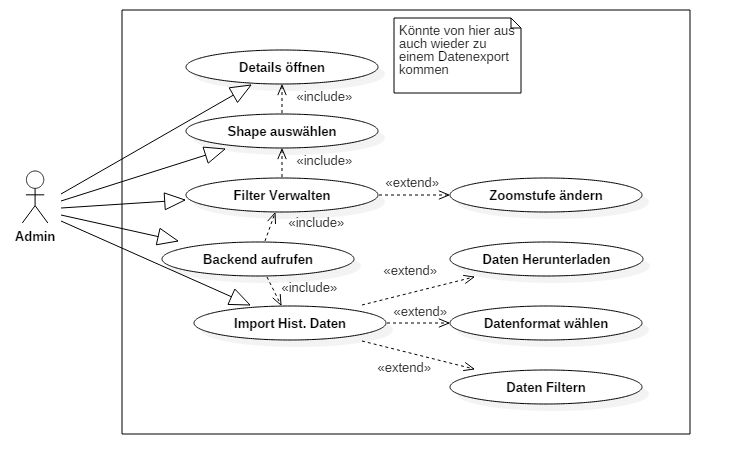
\includegraphics[width=1\linewidth]{diagrams/UseCaseDiagram1.png}
       
       Dieser Anwendungsfall beschreibt die Bedienung des Webinterface. Dem Nutzer stehen folgende Aktionen zur Verfügung:
       \begin{itemize}
            \item Karte anzeigen
            \item Anzeige anpassen
            \item Daten exportieren
            \item Export anpassen
        \end{itemize}
        Nachdem der Nutzer auf das Webinterface zugreift, kann er sich die Karte anzeigen lassen. Diese visualisiert die Daten, welche 
        vom Server bereitgestellt werden. Die Anzeige der Karte, sowie des gesamten Interfaces lässt sich an die Wünsche des Nutzers 
        anpassen, beispielsweise durch die Einbeziehung von Graphen zur besseren Darstellung. Die Datenbestände lassen sich 
        herunterladen und in das gewünschte Format exportieren. Durch Beschränkung der Datenmengen auf bestimmte Zeitintervalle, 
        Datentypen und Wertebereiche kann der Export weiter angepasst werden.
        
    % Anwendungsfall Admin-GUI
    \subsection{Bedienung der Admin-GUI}
        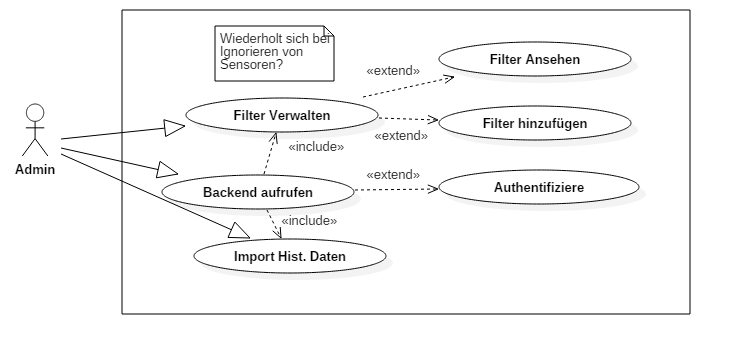
\includegraphics[width=1\linewidth]{diagrams/UseCaseDiagram2.png}
        
        Dieser Anwendungsfall beschreibt die Bedienung der Admin-GUI. Dem Admin stehen folgende Aktionen zur Verfügung:
        \begin{itemize}
            \item Authentifikation
            \item Serverwartung
            \item DataStreams importieren
            \item Sensoren ignorieren
        \end{itemize}
        Um Zugriff auf die Funktionen des Admin-GUIs zu erhalten, muss sich der Admin zunächst authentifizieren. War dies erfolgreich, so 
        kann der Server gewartet werden. Der Admin kann ihn starten sowie beenden um Analysen durchzuführen und eventuelle 
        Fehler zu beheben. Weiterhin lassen sich DataStreams importieren, wodurch der Server diese verarbeiten und weiterverbreiten 
        kann. Dadurch können auch historische Datenbestände in den Datensatz aufgenommen werden. Auch hat der Admin die 
        Möglichkeit auszuwählen, welche Sensoren ignoriert werden, also wessen Daten nicht verbreitet und in den Datenbestand 
        aufgenommen werden sollen.
        
\section{Aktivitätsdiagramm}
    % Aktivitätsdiagramm
    \subsection{}
        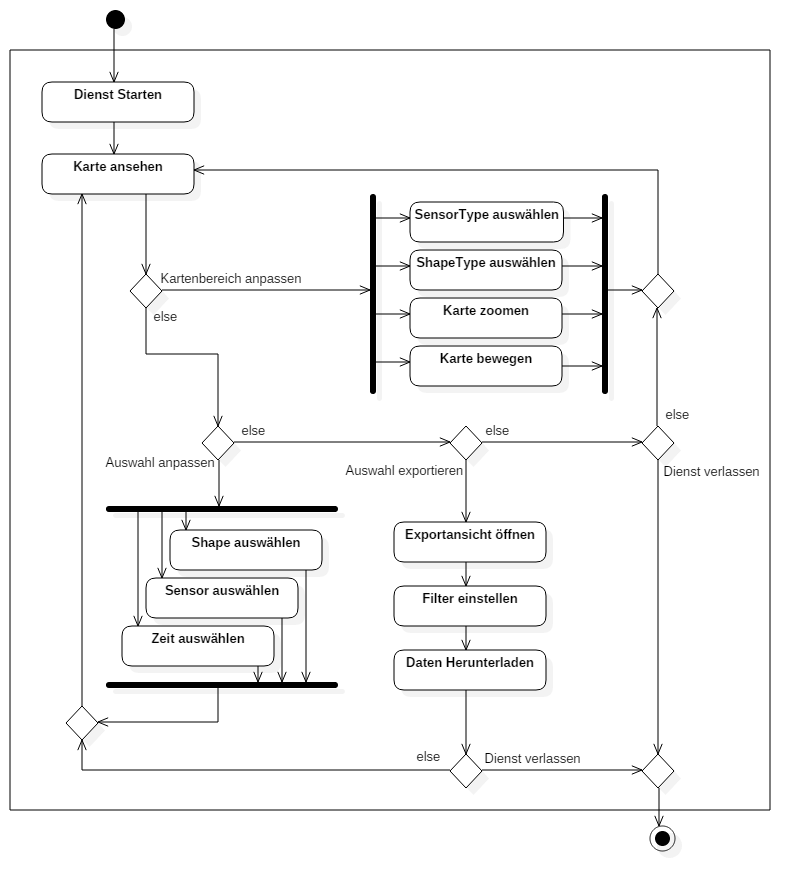
\includegraphics[width=1\linewidth]{diagrams/ActivityDiagram1.png}
        
        Das Aktivitätsdiagramm beschreibt das Verhalten des Webdienstes, der durch das Laden der Dienstwebseite gestartet wird und durch Schließen des Tabs indem er geladen wurde wieder beendet wird.
        
        Jegliche Interaktion mit dem Dienst findet auf derselben Ansicht statt. Es ist keine Reihenfolge für die möglichen Aktionen vorgegeben. So kann unabhängig voneinander der Kartenbereich oder die Auswahl (Selektion) angepasst werden. Das gleiche gilt für das Anfordern eines Downloads allgemeiner oder selektierter Daten.
        
        Die Kartendarstellung kann angepasst werden, sodass die gewünschte Anzeige erreicht wird:
        \begin{itemize}
            \item SensorType auswählen
            \item ShapeType/ClusterType auswählen
            \item Kartenbereich zoomen
            \item Kartenbereich verschieben
        \end{itemize}

        Die Selektion kann angepasst werden:
        \begin{itemize}
            \item Selektion eines Shapes/Clusters
            \item Selektion eines Sensors
            \item Selektion eines Datums
        \end{itemize}

        Daten können exportiert werden. Dazu kann entweder die letzte Selektion verwendet werden. Alternativ wird über Filter der gewünschte Datensatz eingegrenzt. Darauf folgt dann der Download der Daten.


        
